\subsection*{AFTer-UNet: Axial Fusion Transformer UNet for Medical Image Segmentation}

% \subsection*{Ссылка} \url{https://arxiv.org/abs/2110.10403}
\subsubsection*{Введение}
Последние достижения в моделях, основанных на трансформерах 
притянули внимание исследователей для изучения данных техник 
в сегментации медицинских изображений. Особенно часто трансформеры используются 
совместно с  U-Net \cite{Unet} подобными моделями (и их производными), которые показали 
хороший результат в обработке двумерных и трехмерных изображений.
В существующих методах, основанных на двумерных изображениях, 
сверточные слои напрямую заменяются трансформерами, либо трасформер применяется в 
качестве дополнительного промежуточного энкодера между энкодером и декодером U-Net. 
Однако, при таком подходе пространственная информация используется не полностью, сеть 
видит только срезы трехмерного изображения, не учитывая связи в целом трехмерном изображении.

\subsubsection*{Основная идея}
Для того, чтобы трансформер мог находить связи между признаками, 
находящимися на далеком расстоянии в трехмерных медицинских изображениях,
в данной работе предлагается архитектура Axial Fusion Transformer UNet (AFTer-UNet).
AFTer-UNet \cite{ATerUnet} следует архитектуре U-Net, которая состоит из двумерного сверточного энкодера 
и декодера, но между ними авторы разместили промежуточный axial fusion transformer энкодер, 
для того, чтобы связать контекстную информацию из соседних срезов. Промежуточный 
энкодер снижает вычислительную сложность тем, что сначала отдельно вычисляется 
фокус (attention) вдоль осей и внутри одного среза, а потом полученная ифнормация 
объединяется для составления финальной карты сегментации.
\\
\begin{minipage}{1.0\linewidth}
    \begin{center}
        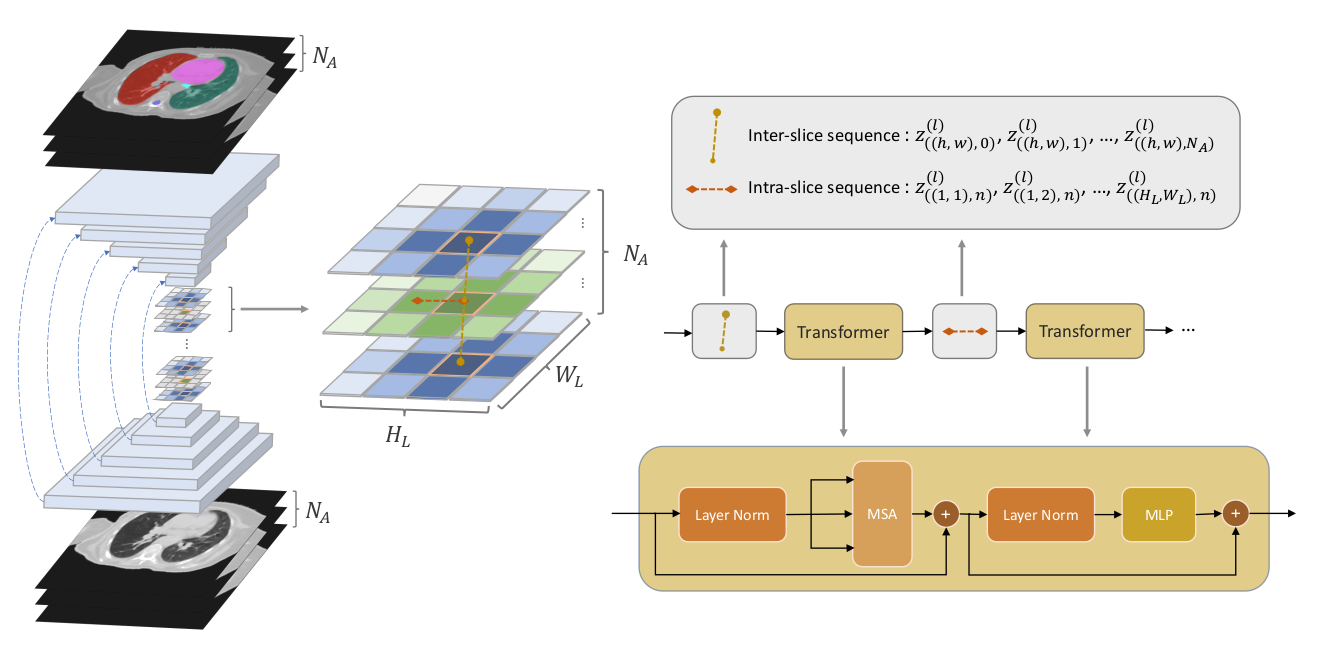
\includegraphics[scale=0.3]{ann20_arch.png} \\
        % \caption{\scriptsize{
        %     Архитектура AFTer-UNet.
        % }}
    \end{center}
    
\end{minipage}
\subsubsection*{Данные}
BCV, Thorax-85, SegTHOR
\subsection*{Результаты}

\begin{minipage}{1.0\linewidth}
    \begin{center}
        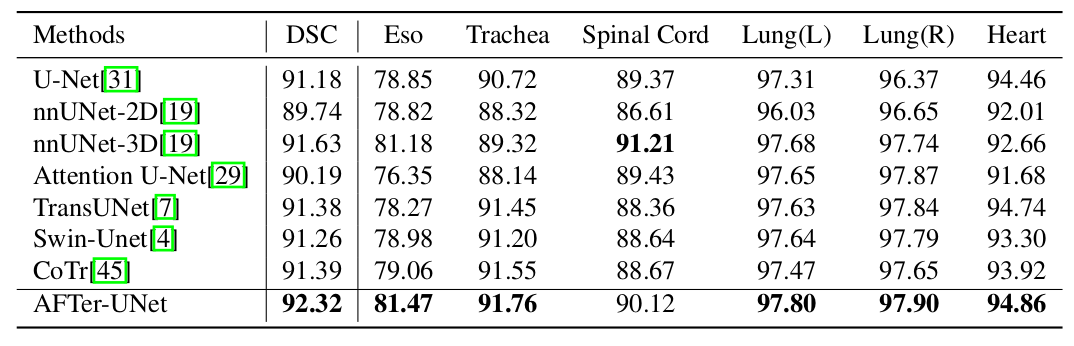
\includegraphics[scale=0.35]{ann20_res1.png} \\
        % \caption{\scriptsize{
        %     Dice score различных методов на датасете Thorax-85.
        % }}
    \end{center}
    
\end{minipage}
\\
\begin{minipage}{1.0\linewidth}
    \begin{center}
        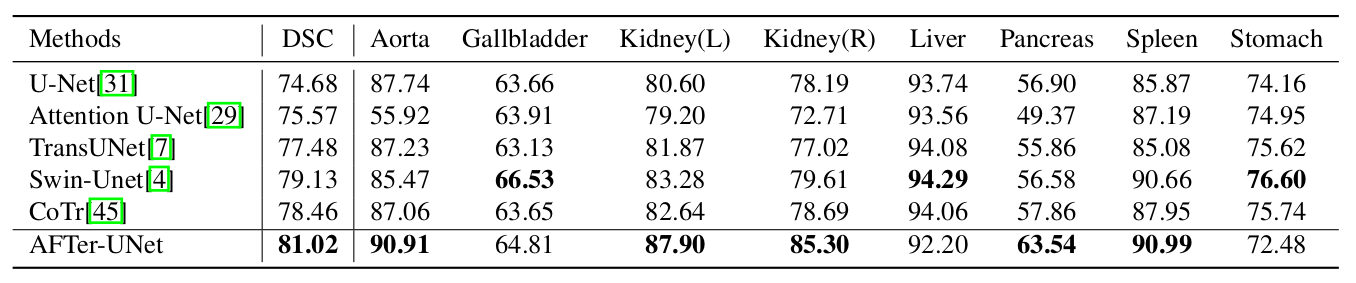
\includegraphics[scale=0.35]{ann20_res2.png} \\
        % \caption{\scriptsize{ 
        %     Dice score различных методов на датасете BCV.}}
    \end{center}
    
\end{minipage} 

\subsubsection*{Заключение}
Был предложен новый фреймворк AFTer-UNet для решения задачи сегментации 
трехмерных медицинских изображений, в котором благодаря промежуточному энкодеру
снижена вычислительная сложность. По результатам проведения экспериментов 
AFTer-UNet показала лучшие результаты по сравнению с существующими моделями, использующими
трансформеры.